\section{Prueba $\chi-$cuadrada}

La \emph{prueba $\chi^{2}$} se usa comúnmente para comparar \emph{datos observados vs datos esperados} suponiendo que los datos siguen ciertas hipótesis.


Debemos suponer cierta hipótesis, la cuál nuestros datos seguirán y calculamos los datos esperados de acuerdo a esa hipótesis.


Debemos ya tener los datos observados, y calcular la desviación entre estos y los esperados usando el estadístico definido en la siguiente fórmula:
\begin{align}
	\texttt{valor }\chi^{2}\texttt{:} g= \sum\dfrac{\left( O-E \right)^{2}}{E},
\end{align}
donde $O$ es el valor observado y $E$ el esperado, con la suma sobre todos los posibles datos.

\paragraph{Aplicaciones del estadístico $\chi-$cuadrada}
La prueba de ji cuadrado se puede usar para hacer lo siguiente:
\begin{itemize}
	\item Mostrar una relación causal o independencia entre una variable de entrada y otra de salida.  
	\item Verificar si los datos observados provienen de una fuente justa / imparcial. 
	\item Comproblemaar si los datos son demasiado buenos para ser verdad.
\end{itemize}


\paragraph{Ejemplo}
Realicemos un experimento hipotético en el que una moneda se lanza 10 veces. ¿Cuántas veces espera obtener ya sea un reverso o un sol?  La respuesta adecuada sería 5.  Ahora bien, ¿qué pasaría si realizamos este experimento 1000 veces y registramos los números de reversos y soles.


Supongamos que observamos soles 553 veces y reversos el resto de ocasiones:
\begin{center}
	$H_{0}:$ La proporción de soles y reversos es $0.5$ \\
	$H_{a}:$ La proporción no es $0.5$
\end{center}



\begin{center}
	\begin{tabular}{|l|l|l|}\hline
		& Soles & reversos\\\hline
		Observado & 553 & 447\\\hline
		Esperado & 500 & 500\\\hline
	\end{tabular}
\end{center}


Calculemos el valor $\chi^{2}:$
\begin{align}
	g = \dfrac{\left( \left( 553-500 \right)^{2}+\left( 447-500 \right)^{5} \right)}{500}\approx 11.236
\end{align}



Este valor$-\chi^{2}$ se compara al valor en una \emph{distribución $\chi^{2}$} para un número dado de \emph{grados de libertad} y un nivel de significación.

\paragraph{La Distribución $\chi^{2}$}
Sean $X_{1},X_{2},...,X_{\nu}$ variables aleatorias independientes $N(0,1).$
Consideremos la variable aleatoria
\begin{align}
	\label{outline:19}
	\chi^{2}=X_{1}^{2}+...+X_{\nu}^{2}
\end{align}
a la que llamaremos \emph{chi cuadrada.} Su correspondiente distribución de problemaabilidad recibe el mismo nombre.

\paragraph{Propiedades de $\chi^{2}$}
\begin{align}
	\label{eq:22}
	\mu=\nu, \; \s = 2\nu
\end{align}


[]{scipy.stats.chi2}
\begin{lstlisting}[language=Python]
	from scipy.stats import chi2
	import numpy as np
	import matplotlib.pyplot as plt
	fig, ax = plt.subplots(1, 1)
	
	df = 55
	
	x = np.linspace(chi2.ppf(0.01, df),
	chi2.ppf(0.99, df), 100)
	ax.plot(x, chi2.pdf(x, df),'r-',
	lw=5, alpha=0.6, label='chi2 pdf')
\end{lstlisting}



\begin{figure}
	\centering
	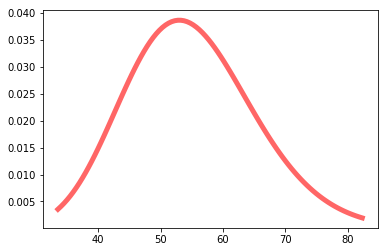
\includegraphics[height=5cm,keepaspectratio=true]{./images/statsChi2.png}
	% statsChi2.png: 0x0 pixel, 300dpi, 0.00x0.00 cm, bb=
	\caption{Función de densidad de distribución $\chi^2$ con $\nu=55$}
	\label{fig:Chi2}
\end{figure}


[]{\texttt{statsChi2.py}}
\begin{lstlisting}[language=Python]
	from scipy.stats import chi2
	import numpy as np
	import seaborn as sns
	import matplotlib.pyplot as plt
	
	sns.set_palette("husl")
	fig, ax = plt.subplots(1, 1)
	
	for df in range(2,15+1):
	x = np.linspace(chi2.ppf(0.01, df),
	chi2.ppf(0.99, df), 100)
	ax.plot(x, chi2.pdf(x, df), label='chi2 pdf')
\end{lstlisting}



\begin{center}
	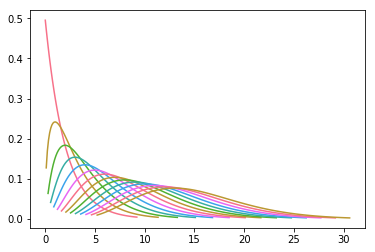
\includegraphics[height=7cm,keepaspectratio=true]{./images/statsChi2Several.png}
	% statsChi2Several.png: 0x0 pixel, 300dpi, 0.00x0.00 cm, bb=
\end{center}


\paragraph{Regresando a nuestro ejemplo...}
El número de grados de libertad es el número de categorías menos uno.  En nuestro ejemplo $\nu = 2-1 =1.$  Supongamos un nivel de significación $\beta=0.05.$


\begin{figure}
	\centering
	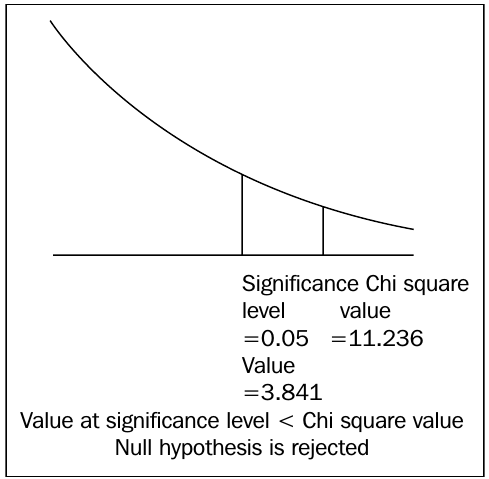
\includegraphics[height=5cm,keepaspectratio=true]{./images/kum0407.png}
	% kum0407.png: 0x0 pixel, 300dpi, 0.00x0.00 cm, bb=
	\caption{La hipótesis nula se rechaza porque el valor del estadístico $\chi^2$ al nivel de significación es menor que el valor del estadístico.}
	\label{fig:0407}
\end{figure}


[]{Otro ejemplo}
Examinemos otros ejemplo donde queremos demostrar que el género de un estudiante y las materias que escoge son independientes.


Supongamos que un grupo de estudiantes, la siguiente tabla representa el número de hombres y mujeres que toman matemáticas, arte y comercio como sus materias principales.


\begin{center}
	\begin{tabular}{|l|l|l|l|l|}\hline
		& Matemáticas & Artes & Comercio & Total\\\hline
		Hombres & 68 & 52 & 90 & 210\\\hline
		Mujeres & 28 & 37 & 35 & 100\\\hline
		Total & 106 & 89 & 125 & 310\\\hline
	\end{tabular}
\end{center}



Si en la elección de las materias, no fuera relevante el género, entonces el número esperado de hombres y mujeres tomando diferentes materias sería
\begin{center}
	\begin{tabular}{|l|l|l|l|l|}\hline
		& Matemáticas & Arte & Comercio & Total\\\hline
		Niños &  &  &  & \\\hline
		Niñas &  &  &  & \\\hline
		Total &  &  &  & \\\hline
	\end{tabular}
\end{center}



Las desviaciones se calculan usando la fórmula
$(O-E)^2/E$:
\begin{center}
	\begin{tabular}{|l|l|l|l|l|}\hline
		& Matemáticas & Arte & Comercio & Total\\\hline
		Hombres &  &  &  & \\\hline
		Mujeres &  &  &  & \\\hline
		Total &  &  &  & \\\hline
	\end{tabular}
\end{center}

El estadístico $\chi^{2}$ se obtiene al sumar todos estos valores.

\paragraph{Conclusiones (del profesor)}
Como $\chi^{2}= 4.99$ y el valor del estadístico $\chi^{2}$ a un nivel se significación es $11.07,$ la hipótesis nula se acepta.

De manera equivalente
\begin{align}
	\texttt{valor-}p=1- F_{\chi^{2}}(4.99)=0.416991040312>\beta=0.05,
\end{align}
obtenemos la misma conclusión:
\begin{center}
	\emph{La elección de materias es independiente del género.}
\end{center}


